\documentclass[12]{article}
\usepackage{listings}
\usepackage{float}
\usepackage{amsmath}

\usepackage{graphicx}
\usepackage{tikz}
\usepackage{algorithm}
\usepackage{geometry}

\geometry{
  a4paper,
  total={210mm,297mm},
  left=20mm,
  right=20mm,
  top=20mm,
  bottom=20mm,
}


\title{\textbf{CSCI 6650 – Intelligent Agents\\Spring'23}\\\textbf{Homework-5}}
\author{Sharmin Aktar, 2581728}

\date{}
\begin{document}

\begin{figure}
\centering

\includegraphics[width=0.5\textwidth]{images/uno_logo.png}
\end{figure}

\maketitle

\section*{Question and Answer}

\subsection*{\textbf{Question 1}}
\textbf{What is a $C$-space? What is the $C$-space for a car?}


\subsection*{Answer}

In robotics, the $C$-space (short for configuration space) is a mathematical representation of all possible configurations of a robot in its environment. It is a manifold of dimension $n$, where $n$ is the number of degrees of freedom of the robot. The $C$-space provides a powerful abstraction that enables motion planning algorithms to conduct a search in the $C$-space to find a collision-free path for the robot to move from its initial position to its goal position.

For a car, the $C$-space would be the set of all possible positions and orientations of the car's wheels and body in its environment. The dimension of the $C$-space for a car would depend on the number of degrees of freedom of the car's motion, which could include the position and orientation of each wheel, the steering angle, and the overall position and orientation of the car's body.



\subsection*{\textbf{Question 2}}
\textbf{What is SO(3)? How to compute distances in SO(3)?}

\subsection*{Answer}

SO(3) is the special orthogonal group of 3-dimensional rotations. It consists of all $3\times3$ matrices with determinant 1 and orthogonal columns, which represent proper rotations in 3D space.

To compare rotations in SO(3) using the $h=(a,b,c,d)$ quaternion representation, we can use the following distance metric:

\begin{equation*}
\rho_s(h_1, h_2) = \cos^{-1}(a_1a_2 + b_1b_2 + c_1c_2 + d_1d_2)
\end{equation*}

where $h_1$ and $h_2$ are two quaternions representing two rotations in SO(3).

However, we need to take into account the identification of antipodal points in SO(3). This means that if $h$ represents a rotation, then $-h$ represents the same rotation but with an opposite direction. Therefore, we need to consider the distance between $h_1$ and both $h_2$ and $-h_2$, and take the minimum of the two:

\begin{equation*}
\rho(h_1, h_2) = \min(\rho_s(h_1, h_2), \rho_s(h_1, -h_2))
\end{equation*}

There are other possibilities for computing distances in SO(3) besides the geodesic distance and the quaternion distance.

One possibility is to use the Euclidean distance in yaw-pitch-roll space. In this representation, a rotation matrix is parameterized by three angles: yaw, pitch, and roll. The Euclidean distance between two rotations can then be computed as the Euclidean distance between their corresponding yaw-pitch-roll angles.

Another possibility is to use the Euclidean distance in the space of $3\times3$ matrices, denoted by R9. In this representation, a rotation matrix is treated as a point in R9, where each element of the matrix is a coordinate in R. The Euclidean distance between two rotation matrices can then be computed as the Euclidean distance between their corresponding points in $\mathbf{R}^9$.


\subsection*{\textbf{Question 3}}
\textbf{what is homeomorphism? Give some examples for homeomorphic and non-homeomorphic subspaces?}


\subsection*{Answer}


Homeomorphism is a fundamental concept in topology that allows us to define when two topological spaces are equivalent. Two topological spaces $X$ and $Y$ are said to be homeomorphic, denoted by $X \cong Y$, if there exists a bijective (one-to-one and onto) function $f: X \to Y$ such that both $f$ and its inverse $f^{-1}$ are continuous. In other words, a homeomorphism is a continuous deformation that can transform one topological space into another without tearing or gluing.




\textbf{Examples of homeomorphic subspaces:}

\begin{itemize}
\item The open interval $(0,1)$ and the open interval $(0,5)$ are homeomorphic via the function $f(x) = 5x$.
\item The sets $(0,1)$ and $(1,\infty)$ are homeomorphic via the function $f(x) = \frac{1}{x}$.
\item The set $(-1,1)$ is homeomorphic to all of $\mathbb{R}$ via the function $f(x) = \frac{2 \tan^{-1}(x)}{\pi}$.
\end{itemize}

\textbf{Examples of non-homeomorphic subspaces:}

\begin{itemize}
\item The closed interval $[0,1]$ and the open interval $(0,1)$ are not homeomorphic.
\item The closed interval $[0,1]$ and the half-open interval $[0,1)$ are not homeomorphic.
\end{itemize}

\begin{figure}[h]
\centering
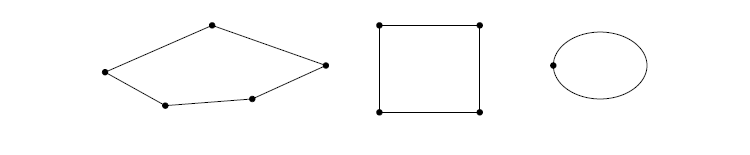
\includegraphics[scale=0.5]{images/homeomorphic_graphs_1.png}
\caption{Even though the graphs are not isomorphic, the corresponding topological spaces may be homeomorphic due to useless vertices. The example graphs map into $\mathbb{R}^2$, and are all homeomorphic to a circle.}
\label{fig:homeomorphic_graphs_1}
\end{figure}

\begin{figure}[h]
\centering
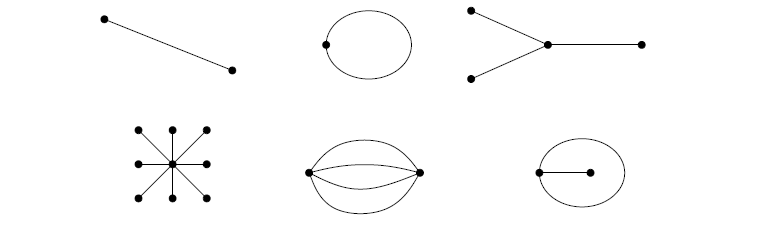
\includegraphics[scale=0.5]{images/homeomorphic_graphs_2.png}
\caption{These topological graphs map into subsets of $\mathbf{R}^2$ that are not homeomorphic to each other.}
\label{fig:homeomorphic_graphs_2}
\end{figure}

It is important to note that closed and open sets can behave differently under homeomorphisms. For example, the endpoints of a closed interval can cause trouble when trying to construct a bijective continuous function. However, bounded and unbounded sets can still be homeomorphic. Linear transformations can also be used to define homeomorphisms. If a subset $X \subset \mathbb{R}^n$ can be mapped to another subset $Y \subset \mathbb{R}^n$ via a nonsingular linear transformation, then $X$ and $Y$ are homeomorphic.



\end{document}
